
\subsection{Operads}

Our goal in this paper was to present an elementary method to formalize quantum
computing in the language of TQFTs and geometric structures supported on them.
Hence our constructions are mostly based on combinatorial and geometric data
that can be associated with cobordisms. Nevertheless, one cannot but notice the
similarity of transport graphs and, more visibly, cobordisms themselves with
operads. As a start, consider the operad of rooted trees whose non-root vertices
are all leaves and where composition is given by gluing the root of a tree with
one of the leaves of another \cite{WhatOp}. Of course, for each leaf, we get a
different composite which is different from gluing of cobordisms, at first
sight. An example is shown below, where the subscript of the composition sign
indicates the leaf chosen for the gluing.
\[\begin{tikzpicture}

\colvert{black}{-2, 0}{a}
\colvert{black}{-3, 0.5}{a1};
\colvert{black}{-3, 0}{a2};
\colvert{black}{-3, -0.5}{a3};
\draw (a1) -- (a);
\draw (a2) -- (a);
\draw (a3) -- (a);

\lblvert{-1.5, 0}{comp}{$\circ_2$}

\colvert{black}{0, 0}{a}
\colvert{black}{-1, 0.25}{a1};
\colvert{black}{-1, -0.25}{a2};
\draw (a1) -- (a);
\draw (a2) -- (a);

\lblvert{0.5, 0}{eq}{$=$}

\colvert{black}{3, 0}{a}
\colvert{black}{2, 0.5}{a1};
\colvert{black}{2, 0}{a2};
\colvert{black}{2, -0.5}{a3};
\draw (a1) -- (a);
\draw (a2) -- (a);
\draw (a3) -- (a);

\colvert{black}{1, 0.25}{a4};
\colvert{black}{1, -0.25}{a5};
\draw (a4) -- (a2);
\draw (a5) -- (a2);

\end{tikzpicture}
\]

However, we notice that the difference of this situation with transport graphs
or cobordisms is artificial for we could define composition operations for
transport graphs and cobordisms parametrized by their inputs and outputs just as
in the case of operads. Note, however, that we need to handle the gluing of
multiple outputs to inputs in various combinations. For this, we informally
introduce a modification of operads.

\begin{defn}
Let $\s{C}$ be any (not necessarily symmetric) monoidal category and
$P = \set{P(n, m)}_{n, m \in \N}$ be a
collection of objects of $\s{C}$. For any $n \in \N$ and $1 \leq i \leq n$,
let $I = \set{i, i + 1, \dots, i + m} \subset \set{1, \dots, n}$. For each
such $n$ and $I$ as well as some $n' \in \N$, suppose there is a morphism in
$\s{C}$ as follows:
\[
  \circ_I : P(n, m) \tensor P(n', n) \to P(n', m)
\]
Then, with some coherence conditions we have not explored, we will call
$P$ a multioperad in $\s{C}$.
\end{defn}

\begin{exm}
Consider the same diagram above giving an example of operads of trees. This
diagram is an example of a (pre)transport graph if we direct the edges and
colour the vertices! The only difference is that the composition operation given
here is parametrized by a ``segment'' of the gluing site. We give another
example below:
\[\begin{tikzpicture}

\colvert{green!55!black}{1, 2.5}{c}
\colvert{blue!55!black}{1, 1.75}{cc}
\colvert{blue!55!black}{0, 3.25}{c1}
\colvert{green!55!black}{0, 2.75}{c2}
\colvert{blue!55!black}{0, 2.25}{c3}
\colvert{blue!55!black}{0, 1.75}{c4}
\midarrow{c1}{c}
\midarrow{c2}{c}
\midarrow{c3}{c}
\midarrow{c4}{c}
\midarrow{c4}{cc}

\lblvert{2, 2.5}{comp}{$\circ_{\set{2, 3}}$}

\colvert{green!55!black}{4, 3}{a}
\colvert{blue!55!black}{3, 3.5}{a1}
\colvert{blue!55!black}{3, 3}{a2}
\colvert{blue!55!black}{3, 2.5}{a3}
\midarrow{a1}{a}
\midarrow{a2}{a}
\midarrow{a3}{a}

\colvert{blue!55!black}{4, 2}{b}
\colvert{green!55!black}{3, 2}{b1}
\colvert{blue!55!black}{3, 1.5}{b2}
\midarrow{b1}{b}
\midarrow{b2}{b}
\midarrow{a3}{b}

\lblvert{5, 2.5}{comp}{$=$}

\colvert{green!55!black}{8, 2.5}{c}
\colvert{blue!55!black}{8, 1.75}{cc}
\colvert{blue!55!black}{7, 3.25}{c1}
\colvert{green!55!black}{7, 2.75}{c2}
\colvert{blue!55!black}{7, 2.25}{c3}
\colvert{blue!55!black}{7, 1.75}{c4}
\midarrow{c1}{c}
\midarrow{c2}{c}
\midarrow{c3}{c}
\midarrow{c4}{c}
\midarrow{c4}{cc}

\colvert{blue!55!black}{6, 3.5}{a1}
\colvert{blue!55!black}{6, 3}{a2}
\colvert{blue!55!black}{6, 2.5}{a3}
\colvert{green!55!black}{6, 2}{b1}
\colvert{blue!55!black}{6, 1.5}{b2}
\midarrow{a1}{c2}
\midarrow{a2}{c2}
\midarrow{a3}{c2}
\midarrow{b1}{c3}
\midarrow{b2}{c3}
\midarrow{a3}{c3}

\end{tikzpicture}\]
In this example, we considered coloured vertices and hence what we really
require is a coloured variant of multioperads, in the same spirit of introducing
colours to ordinary operads.
\end{exm}

\begin{exm}
Of course, thick tangles admit the same structure -- simply interpret the above
example in the context of thick tangles.
\end{exm}

Note, in particular, the similarity with cyclic operads as defined in
\cite{ModOp}. Recall that a cyclic operad $P$ is roughly an operad with the
action of the symmetric group $S_n$ group on $P(n)$ replaced by an action of
$S_{n + 1}$. This effectively conflates the ``inputs'' and ``outputs'' of an
operad ``element''. Here, however, we take a much more elementary approach --
simply allow multiple inputs and multiple outputs. The other difference is that
a multioperad should not require symmetry in a monoidal category for our
categories of thick tangles and transport graphs are not equipped with symmetry.
We also note a connection to modular operads \cite{ModOp}.

A modular operad is roughly a cyclic operad which allows for the gluing of
``inputs'' and ``outputs'' of the same operation \cite{Giansiracusa}.
This exact formalism is not present in the our setting, but we can introduce
something similar, although in a non-unique way. Consider the simple example
below. Here, we wish to glue the first and only output to the first input, say.
One way to accomplish this is shown on the right.
\[\begin{tikzpicture}
\colvert{green!55!black}{0, 3}{a}
\colvert{blue!55!black}{-1, 3.5}{a1}
\colvert{blue!55!black}{-1, 3}{a2}
\colvert{blue!55!black}{-1, 2.5}{a3}
\midarrow{a1}{a}
\midarrow{a2}{a}
\midarrow{a3}{a}

\draw[->] (1, 3) to (2, 3);

\colvert{blue!55!black}{5, 3}{a}
\colvert{green!55!black}{4, 3.5}{a1}
\colvert{blue!55!black}{4, 3}{a2}
\colvert{blue!55!black}{4, 2.5}{a3}
\midarrow{a1}{a}
\midarrow{a2}{a}
\midarrow{a3}{a}

\colvert{green!55!black}{3, 4}{b}
\colvert{green!55!black}{6, 4}{c}
\midarrow{b}{a1}
\midarrow{b}{c}
\midarrow{a}{c}
\end{tikzpicture}\]

We observe that these gluing constructions work as-is for the gluing
construction for bundles with connection as well so that our framework for
quantum computing could be treated in this operadic formalism but we will not
explore this idea in greater detail in this paper. Nevertheless,
these preliminary observations hint at various possibilities.
Modular operads as developed by Getzler and Kapranov generalize
Kontsevich's graph complexes \cite{ModOp}. It if of interest to fully flesh out
the connection of transport graphs to modular operads for this could lead to the
application of Chern-Simons theory to the quantum computing framework
developed in this paper. On the other hand, an approach to cobordism
theory using coloured operads \cite{CobOp} has been used to categorify $sl_n$
quantum invariants. The operadic approach to transport graphs on manifolds
with connections might be one way to relate categorification in
representation theory with quantum computing.

